% vim:spelllang=uk,en
\documentclass[simple,14pt,utf8,ukrainian]{eskdtext}
\usepackage{eskddstu}

\usepackage{cmap}
\usepackage[T2A]{fontenc}
\usepackage[utf8]{inputenc}
% \usepackage{concrete}
\usepackage{pscyr}
\usepackage{cite}
\usepackage{url}

\usepackage{textcase}

\usepackage{lscape}

\pdfcompresslevel=9 % сжимать PDF
\usepackage{pdflscape} % для возможности альбомного размещения некоторых страниц
\usepackage[pdftex]{hyperref}
% настройка ссылок в оглавлении для pdf формата
\hypersetup{unicode=true,
            pdftitle={Диплом},
            pdfauthor={Погода Михайло},
            pdfcreator={pdflatex},
            pdfsubject={},
            pdfborder    = {0 0 0},
            bookmarksopen,
            bookmarksnumbered,
            bookmarksopenlevel = 2,
            pdfkeywords={},
            colorlinks=true, % установка цвета ссылок в оглавлении
            citecolor=black,
            filecolor=black,
            linkcolor=black,
            urlcolor=blue}

\usepackage{amsmath}
\usepackage{amssymb}
\usepackage{moreverb}
\usepackage{indentfirst}
\usepackage{misccorr}

\usepackage{xtab}
\usepackage{nccfoots}
\usepackage{nccstretch}
\usepackage{siunitx}
\usepackage{multirow}

\begin{document}
% \ESKDstyle{empty}
\tableofcontents
\clearpage
\section{Охорона праці}\label{sec:WS}
  За сучасних умов, комп’ютери набули широкого поширення.
  Вони застосовується на кожному підприємстві для організації діяльності
  праці.
  Комп’ютери є невід’ємним і, найчастіше, одним із головних інструментів при
  виконанні поставлених завдань.

  Даних розділ дипломної роботи носить рекомендаційний характер та має
  відношення до робіт одного типу, а отже подальші рекомендації будуть
  пов’язані зі специфікою роботи з персональними комп’ютерами.

  Основним нормативним документом щодо забезпечення охорони праці користувачів
  персонального комп’ютера є НПАОП~0.00-1.28-10 та
  ДНАОП~0.00-1.31-99\cite{about-work-safety}.
  \subsection{Характеристика робочого місця}
    Робоче приміщення знаходиться на четвертому поверсі в цегляному будинку.
    Найближчі будівлі знаходяться на значній відстані та не впливають на
    рівень проникнення світла.
    План приміщення зображений на рис.~\ref{fig:plan}.
    \begin{figure}[ht]
      \centering
      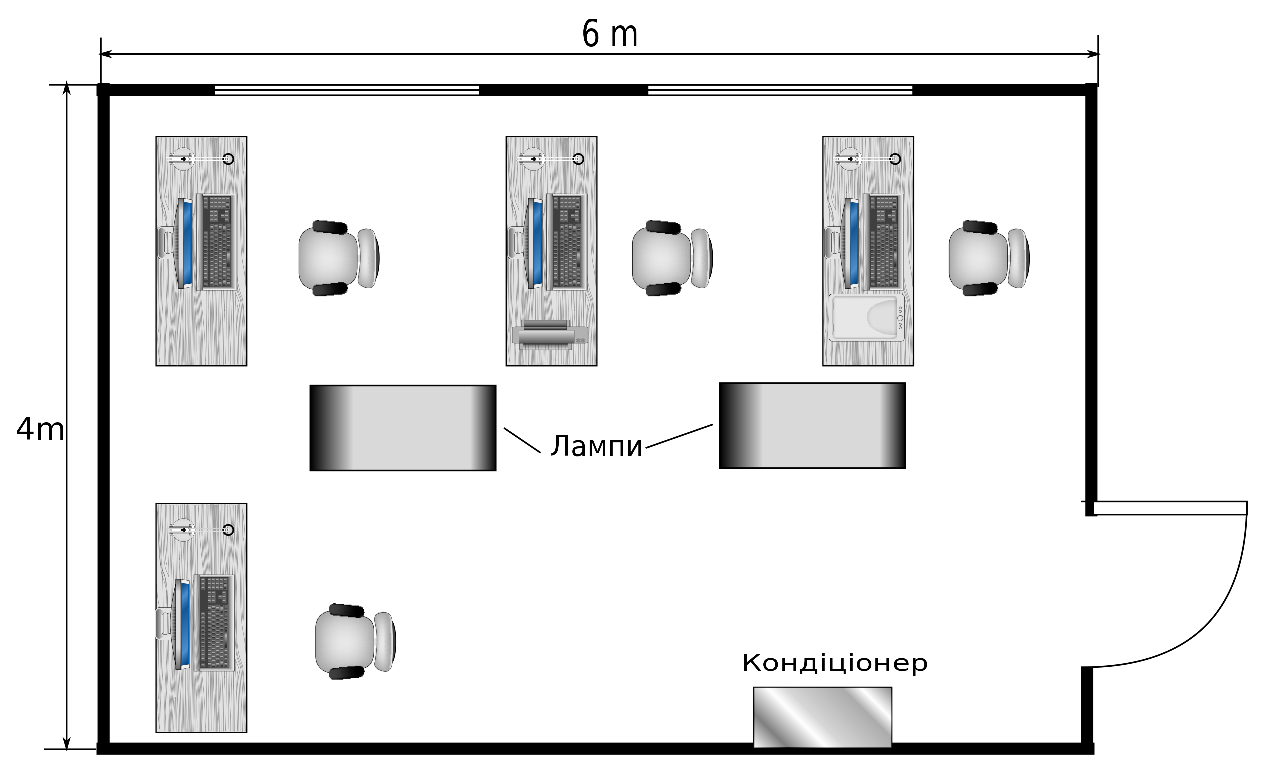
\includegraphics[width=\linewidth]{plan2.eps}
      \caption{План приміщення}
      \label{fig:plan}
    \end{figure}

    Санітарно"=гігієнічні вимоги щодо влаштування приміщень, в яких працівники
    працюють на персональних комп’ютерах, параметрів виробничого середовища,
    організації та обладнання робочих місць, режимів праці та відпочинку при
    роботі з відеотерміналами (ВДТ) і профілактичних медоглядів наведено у
    ДСанПіН 3.3.2.007-98 <<Гігієнічні вимоги до організації роботи з
    візуальними дисплейними терміналами електронно"=обчислювальних машин>>,
    затверджених постановою Головного державного санітарного лікаря України
    від 10~грудня~1998~р. \textnumero~7 (далі --- \emph{ДСанПіН 3.3.2.007-98}).

    Згідно з п.~2.3. ДСанПіН~3.3.2-007-98 розмір площі для одного робочого
    місця оператора персонального комп’ютера повинен бути не менше
    \num{6.0}~м$^2$, а об’єм --- не менше \num{20.0}~м$^3$.
    Довжина кімнати --- \num{6.0}~м, ширина --- \num{4.0}~м, висота ---
    \num{2.7}~м.
    Маються також два вікна (\num{2.0}~м~$\times$~\num{1.6}~м), які спрямовані
    на північ.
    Отже, площа приміщення складає
      \[
        S = 6 \times 4 = 24~\text{м}^2,
      \]
    а обсяг
      \[
        V = 24 \times 2.7 = 64.8~\text{м}^2.
      \]
    Кожне робоче місце обладнане електронно"=обчислювальними машинами з
    РК"=моніторами Samsung LN32D403E2DXZA.
    У приміщенні постійно працює до чотирьох чоловік.
    Отже, на кожне робоче місце припадає по \num{6.0}~м$^2$ площі в об’ємі не
    менше, ніж \num{20.0}~м$^3$, що відповідає санітарним нормам.

    Пункт 4.4. передбачає, що при розміщенні робочих столів з відеотерміналами
    слід дотримувати такі відстані: між бічними поверхнями ВДТ ---
    \num{1.2}~м, відстань від тильної поверхні одного відеотерміналу до екрана
    іншого відеотерміналу --- \num{2.5}~м.\cite{dsanpin}

    Параметри столу: довжина --- \num{1450}~мм, ширина --- \num{740}~мм,
    висота --- \num{730}~мм.
    Відстань між робочими столами також відповідає санітарним нормам, а саме
    не є меншою, ніє \num{2.0}~м.

    Робочі стільці є підйомно"=поворотні, регульовані за висотою, кутом нахилу
    сидіння та спинки.
    Поверхня сидіння --- плоска, а передній край --- заокруглений.
    Регулювання за кожним із параметрів здійснюється незалежно, легко та
    надійно фіксується.

    Екран ВДТ розташовується на відстані \num{670}~мм до очей користувача, що
    є оптимальною відстанню.
    Саме розташовання екрану ВДТ забезпечує зручність зорового спостереження у
    вертикальній площині під кутом \ang{30}.

    Столи були вибрані з урахуванням наступних умов:
    \begin{itemize}
      \item поверхня столу повинна володіти властивостями, що виключають появу
        відблисків в полі зору програміста;
      \item нижня частина столу повинна бути сконструйована так, щоб працівник
        міг зручно сидіти, не був вимушений підтискати ноги;
      \item висота столу повинна бути вибрана з урахуванням можливості сидіти
        вільно, в зручній позі, при необхідності спираючись на підлокітники;
      \item конструкція столу повинна передбачати наявність висувних ящиків.
    \end{itemize}

    Робоче приміщення, що розглядається, оснащене аптечками першої медичної
    допомоги.

  \subsection{Аналіз шкідливих і небезпечних виробничих факторів}
    \subsubsection{Мікроклімат}
      Висока температура повітря негативно позначається на функціональному
      стані людини.
      Оптимальні та припустимі мікрокліматичні параметри у приміщеннях повинні
      враховувати специфіку технологічного процесу при використанні ПК.
      Зокрема, технічні умови експлуатації багатьох типів комп’ютерів містять
      допустимі робочі діапазони параметрів мікроклімату:
      \begin{itemize}
        \item температура повітря має знаходитись в межах від \num{10} до
          \num{40}$^\circ C$;
        \item відносна вологість має знаходитися в межах від \num{40} до
          \num{90}\%.
      \end{itemize}

      За даними ВООЗ, оптимальні значення температури у приміщенні становлять
      \num{19}--\num{23}$^\circ C$, відносна вологість повітря --- \num{55}\%,
      швидкість руху повітря не повинна перевищувати на рівні обличчя
      \num{0.1}~м/с.
      При відчутному нагрівання поверхонь (більше \num{45}$^\circ C$),
      контактуючих з людиною, передбачаються засоби охолодження або ізоляції.
      Особлива увага приділяється шляхом відводу повітря, щоб виключити
      перегрівання або протяг.

      Згідно з діючими в Україні нормативними документами\cite{gost121005}
      мають місце норми, наведені у табл.~\ref{tab:microclimat}.
      \begin{table}[h]
        \centering
        \begin{tabular}{|c|l|c|}
          \hline
            Період року & Параметр мікроклімату & Величина\\
          \hline
            \multirow{3}{*}{Холодний} & Температура повітря &
            \num{22}--\num{24}$^\circ C$\\
          \cline{2-3}
            & Швидкість руху повітря & до \num{0.1}~м/с\\
          \cline{2-3}
            & Відносна вологість & \num{40}--\num{60}\%\\
          \hline
            \multirow{3}{*}{Теплий} & Температура повітря &
            \num{23}--\num{25}$^\circ C$\\
          \cline{2-3}
            & Швидкість руху повітря & \num{0.1}--\num{0.2}~м/с\\
          \cline{2-3}
            & Відносна вологість & \num{40}--\num{60}\%\\
          \hline
        \end{tabular}
        \caption{Параметри мікроклімату для приміщень, де встановлені
        комп’ютери}
        \label{tab:microclimat}
      \end{table}

      Завдяки встановленого кондиціонера можливо індівідуальне регулювання
      роздачі повітря в приміщенні.

      В процесі роботи змінюється концентрація іонів у повітрі робочої зони.
      Нормалізуючий вплив на аероіонний склад повітря робочої зони
      забезпечують: примусова вентиляція, захисні екрани та застосування
      іонізаторів.
      Повітря, що надходить у робочі приміщення, має бути очищене від
      забруднень, в тому числі від мікроорганізмів.

      Розрахована місцева система кондиціювання. Для цього визначені надлишки
      явного тепла за загальною методикою:
      \begin{equation}
        Q = S \times h \times q,
        \label{eq:nadlishki}
      \end{equation}
      де $Q$ --- теплопритоки (Вт), $S$ --- площа приміщення (м$^2$), $h$ ---
      висота приміщення (м), $q$ --- коефіцієнт, рівний \num{30}--\num{40}
      Вт/м$^3$ (для південної сторони --- 40 Вт/м$^3$, для північної --- 30
      Вт/м$^3$, в нашому випадку --- 30 Вт/м$^3$).

      Врахуємо тепло, виділюване людьми й електроприладами.
      Вважається, що в спокійному стані людина виділяє \num{0.1}~кВт тепла;
      комп’ютер та принтер --- \num{0.3} кВт; для інших приладів можна
      вважати, що вони виділяють у виді тепла $\frac{1}{3}$ паспортної
      потужності.
      Додав усі тепловиділення і теплопритоки, ми одержимо необхідну
      потужність охолодження.

      Розрахуємо необхідну потужність для нашого приміщення.
      Для компенсації теплопритоків від стін, вікон, підлоги і стелі
      необхідно:\[
      64.8~\text{м}^3 \times 30~\text{Вт/м}^3 = 1.94~\text{кВт}. \]
      Для компенсації тепла, виділюваного людьми і комп’ютером необхідно:
      \[
        0.1~\text{кВт} \times 4 + 6 \times 0.3~\text{кВт}= 2.2~\text{кВт}
      \]

      \begin{equation}
        Q = 1.94 + 2.2 = 4.14~\text{(кВт)}
        \label{eq:q}
      \end{equation}

      Потужність (точніше, потужність охолодження) є основною характеристикою
      будь-якого кондиціонера.
      Серед різних моделей у нашому випадку пасує модель \texttt{RAS-30 CH1}
      фірми HITACHI, яка має потужність по холоду \num{4.14}~кВт.
    \subsubsection{Шум}
      Встановлено, що шум погіршує умови праці, роблячи шкідливий вплив на
      організм людини.
      При тривалому впливі шуму на людину відбуваються небажані явища:
      знижується гострота зору, слуху, підвищується кров’яний тиск, знижується
      увага.
      Сильний тривалий шум може стати причиною функціональних змін
      серцево"=судинної і нервової систем.

      Нормативний рівень шуму не повинний перевищувати \num{50}~дБа\cite{dsn}.

      У приміщенні маються внутрішні джерела постійного шуму: вентилятор
      блоків ПЕОМ(\num{35}~дБа, \num{8}~годин); принтери(\num{48}~дБа,
      \num{2}~години); дисковод(\num{40}~дБа, \num{0.5}~години).
      Зовнішніми джерелами шуму і вібрації в приміщенні є проїжджаючі
      транспортні засоби (\num{40}~дБа, \num{8}~годин).

      Будівельно"=акустичні методи захисту від шуму передбачені будівельними
      нормами і правилами це:
      \begin{itemize}
        \item звукоізоляція конструкції, що обгороджує, ущільнення по
          периметрі притворів вікон і дверей;
        \item звукопоглинаючі конструкції й екрани;
        \item глушителі шуму, звукопоглинаючі облицювання.
      \end{itemize}

      На робочому місці оператора джерелами шуму, як правило, є технічні
      засоби, такі як --- комп'ютер, принтер, вентиляційне устаткування, а
      також зовнішній шум.
      Вони видають досить незначний шум, тому в приміщенні досить
      використовувати звукопоглинання.
      Зменшення шуму, що проникає в приміщення ззовні, досягається ущільненням
      по периметрі притворів вікон і дверей.
      Під звукопоглинанням розуміють властивість акустично оброблених
      поверхонь зменшувати інтенсивність відбитих ними хвиль за рахунок
      перетворення звукової енергії в теплову.
      Звукопоглинання являється досить ефективним заходом щодо зменшення шуму.
      Найбільш вираженими звукопоглинаючими властивостями володіють
      волокнисто"=пористі матеріали: фібролітові плити, скловолокно,
      мінеральна вата, поліуретановий поропласт, пористий полівінілхлорид і
      інші.
      До звуковбирних матеріалів відносяться лише ті, коефіцієнт
      звукопоглинання яких не нижче \num{0.2}.

      Звукопоглинаючі облицювання з зазначених матеріалів (наприклад, мати із
      супертонкого скловолокна з оболонкою зі склотканини потрібно розмістити
      на стелі і верхніх частинах стін).
      Максимальне звукопоглинання буде досягнуто при облицюванні не менш
      \num{60}\% загальної площі поверхонь приміщення.
    \subsubsection{Освітлення}
      Природне світло проникає через бічні світло"=прорізи, зорієнтовані на
      північ, і забезпечує коефіцієнт природної освітленості (КПО) не нижче
      \num{1.5}\%.

      Як джерело світла при штучному освітленні повинні застосовуватися, як
      правило, люмінесцентні лампи типу ЛБ.
      У даному приміщенні застосовуються лампи NORTCLIFFE HF ECO з частотою
      перетворення \num{46}~кГц.
      Яскравість світильників загального освітлення в зоні кутів
      випромінювання від \ang{50} до \ang{90} відносно вертикалі в подовжній і
      поперечній площинах повинна складати не більше \num{200}~кд/м$^2$, а
      захисний кут світильників повинен бути не більшим за \ang{40}\cite{dbn}.

      Рівень освітленості на робочому столі в зоні розташування документів має
      бути в межах \num{300}--\num{500}~лк.
      У разі неможливості забезпечити даний рівень освітленості системою
      загального освітлення допускається застосування світильників місцевого
      освітлення, але при цьому не повинно бути відблисків на поверхні екрана
      та збільшення освітленості екрану більше ніж до \num{300}~лк.

      Розраховуємо загальний світловий потік для освітлення площі робочого
      приміщення:
      \begin{equation}
        F_{n} = \frac{E_n S K_\text{зап} Z}{\eta},
        \label{eq:f-n}
      \end{equation}
      де $E_n$ --- нормоване значення штучної освітленості, $S$ --- площа
      приміщення, $K_\text{зап}$ --- коефіцієнт запасу, $Z$ --- коефіцієнт
      нерівномірності освітлення, $\eta$ --- коефіцієнт використання
      світильника.
      \[ F_{n} = (0.8 \times 24 \times 2 \times 1.5) / 0.55 = 1.2~\text{лм} \]

      Необхідна кількість світильників визначається за формулою:
      \begin{equation}
        n = \frac{F_n}{F_1},
        \label{eq:n}
      \end{equation}
      де, $F_n$ --- потрібний загальний світовий потік, $F_1$ --- світловий
      потік, створюваний одним світильником.
      \[ n = 1.2 / 0.5 = 2~\text{шт} \]
    \subsubsection{Електробезпека}
      Згідно з Правилами улаштування електроустановок (ПУЕ, 2009~р.) дане
      приміщення відноситься до категорії приміщень без підвищеної безпеки.

      Електроживлення однофазне \num{220}~В з глухо"=заземленою нейтраллю,
      виконане 3-х провідних проводом.
      Для підключення обладнання встановлені розетки з заземлюючим контактом.
      Провідники заземлення приєднані до загального контуру заземлення.
      Опір загального становить \num{3}~Ом.
      Заземлення корпусів ЕОМ та іншого обладнання здійснюється через вилку
      підключення о джерела живлення.
    \subsubsection{Пожежна безпека}
      Дане приміщення відноситься до категорії B, класу П-IIа.
      До цієї зони відносяться приміщення, у яких використовуються тверді чи
      волокнисті речовини, нездатні переходити в зважений стан\cite{napb}.
      У приміщенні є пальні речовини: волокнисті(папір), тверді(дерево),
      пластмаси.

      Тому що ПЕОМ мають велику вартість, з огляду на категорію пожежної
      небезпеки приміщення, будинку з використанням ПЕОМ повинні бути I і II
      ступеня вогнестійкості (тобто всі конструктивні елементи повинні бути
      неспаленими).
      Фактично приміщення відповідає цим нормам (основні будівельні матеріали
      --- цегла, бетон, скло).

      У коридорах будинку установлюються пожежні крани.
      Вода використовується для гасіння пожеж у допоміжних службово-побутових
      приміщеннях.
      Пожежні крани розташовують на висоті \num{1.35}~м від підлоги в найбільш
      доступних місцях.

      Для гасіння пожежі в початковій стадії його виникнення в приміщенні
      встановлено 2 вогнегасника: ВП-1(з) (вогнегасник порошковий закачний
      ємністю \num{1.3+-0.08}~л.

      Для запобігання пожежі в приміщенні прийняті такі міри:
      \begin{itemize}
        \item передбачено вільний доступ до мережних рубильників і вимикачів;
        \item інструктаж з пожежної безпеки і періодичний контроль знань про
          правила пожежної безпеки;
        \item встановлені два димових сповіщувача ИПД-1;
        \item заборона використання електронагрівальних приладів;
        \item маються 2 вогнегасник ВП-1(з);
        \item двері на шляху проходження людей відкриваються назовні;
        \item ширина загального коридору, ширина двер, висота двер
          відповідають нормативним значенням ОНТП 24-86;
        \item призначено відповідального за пожежну безпеку в приміщенні.
      \end{itemize}
  \subsection{Інструкція з техніки безпеки}
    Дії працівників у разі виникнення пожежі:
    \begin{itemize}
      \item Про виникнення пожежі в приміщеннях негайно повідомити пожежну
        охорону за міським телефоном 101.
      \item При цьому необхідно назвати адресу, зазначити кількість поверхів
        будівлі, місце виникнення пожежі, обстановку на пожежі, наявність
        людей, а також повідомити своє прізвище.
      \item Вжити (по можливості) заходи на евакуацію людей, гасіння
        (локалізацію) пожежі з використанням первинних засобів пожежегасіння
        та на збереження матеріальних цінностей.
      \item Повідомити про виникнення пожежі керівника (заступників керівника)
        чи відповідальну компетентну посадову особу та чергового охорони.
      \item У разі необхідності, викликати інші аварійно"=рятувальні служби
        (медичну, газорятувальну тощо).
    \end{itemize}
  \bibliographystyle{ugost2008ls}
  \bibliography{src}
\end{document}
